% main=pgfplots.tex

\chapter{Step-by-Step Tutorials}
{%
\tikzset{external/figure name/.add={}{tutorials_}}%


\section{Introduction}

Visualization of data is often necessary and convenient in order to analyze and
communicate results of research, theses, or perhaps just results.

\PGFPlots{} is a visualization tool. The motivation for \PGFPlots{} is that you
as end-user provide the data and the descriptions as input, and \PGFPlots{}
takes care of rest such as choosing suitable scaling factors, scaling to a
prescribed target dimension, choosing a good displayed range, assigning tick
positions, drawing an axis with descriptions placed at appropriate places.

\PGFPlots{} is a solution for an old problem of visualization in \LaTeX{}: its
descriptions use the same fonts as the embedding text, with exactly the same
font sizes. Its direct embedding in \LaTeX{} makes the use of \LaTeX{}'s
powerful math mode as easy as possible: for any kind of axis descriptions up to
user-defined annotations. It features document-wide line-styles, color schemes,
markers\ldots{} all that makes up consistency.

\PGFPlots{} offers high-quality. At the same time, it is an embedded solution:
it is largely independent of 3rd party tools, although it features import
functions to benefit from available tools.

Its main goal is: you provide your data and your descriptions -- and
\PGFPlots{} runs without more input. If you want, you can customize what you
want.



\section{Solving a Real Use Case: Function Visualization}

In this section, we assume that you want to visualize two functions. The first
function is given by means of a data table. The second function is given by
means of a math expression. We would like to place the two results side by
side, and we would like to have ``proper'' alignment (whatever that means).

As motivated, we have one data table. Let us assume that it is as shown below.
%
\begin{codeexample}[code only]
x_0	f(x)
# some comment line
3.16693000e-05	-4.00001451e+00
1.00816962e-03	-3.08781504e+00
1.98466995e-03	-2.88058811e+00
2.96117027e-03	-2.75205040e+00
3.93767059e-03	-2.65736805e+00
4.91417091e-03	-2.58181091e+00
5.89067124e-03	-2.51862689e+00
...
9.89226496e-01	2.29825980e+00
9.90202997e-01	2.33403276e+00
9.91179497e-01	2.37306821e+00
9.92155997e-01	2.41609413e+00
9.93132498e-01	2.46412019e+00
9.94108998e-01	2.51860712e+00
9.95085498e-01	2.58178769e+00
9.96061999e-01	2.65733975e+00
9.97038499e-01	2.75201383e+00
9.98014999e-01	2.88053559e+00
9.98991500e-01	3.08771757e+00
9.99968000e-01	3.99755546e+00
\end{codeexample}
%
Note that parts of the data file have been omitted here because it is a bit
lengthy. The data file (and all others referenced in this manual) are shipped
with \PGFPlots{}; you can find them in the subfolder
\texttt{doc/latex/pgfplots/plotdata}.


\subsection{Getting the Data Into \TeX{}}
\label{sec:tut1:step1}

Our first step is to get the data table into \PGFPlots{}. In addition, we want
axis descriptions for the |x| and |y| axes and a |title| on top of the plot.

Our first version looks like
%
\begin{codeexample}[]
%\documentclass{article}
%\usepackage{pgfplots}
%\pgfplotsset{compat=1.5}

%\begin{document}

\begin{tikzpicture}
\begin{axis}[
    title=Inv. cum. normal,
    xlabel={$x$},
    ylabel={$y$},
]
    \addplot [blue] table {invcum.dat};
\end{axis}
\end{tikzpicture}
%\end{document}
\end{codeexample}

The code listing already shows a couple of important aspects:
%
\begin{enumerate}
    \item As usual in \LaTeX{}, you include the package using
        |\usepackage{pgfplots}|.
    \item Not so common is |\pgfplotsset{compat=1.5}| .

        A statement like this should always be used in order to (a)~benefit
        from a more or less recent feature set and (b)~avoid changes to your
        picture if you recompile it with a later version of \PGFPlots{}.

        Note that \PGFPlots{} will generate some suggested value into your
        logfile (since 1.6.1). The minimum suggested version is
        |\pgfplotsset{compat=1.3}| as this has great effect on the
        positioning of axis labels.
    \item \PGFPlots{} relies on \Tikz{} and \pgfname{}. You can say it is a
        ``third party package'' on top of \Tikz{}/\pgfname{}.

        Consequently, we have to write each \PGFPlots{} graph into a \Tikz{}
        picture, hence the picture environment given by
        |\begin{tikzpicture} ... \end{tikzpicture}|.
    \item Each axis in \PGFPlots{} is written into a separate environment. In
        our case, we chose |\begin{axis} ... \end{axis}| as this is the
        environment for a normal axis.

        There are more axis environments (like the
        |\begin{loglogaxis} ... \end{loglogaxis}| environment for logarithmic
        axes).

        Although \PGFPlots{} runs with default options, it accepts keys. Lots
        of keys. Typically, you provide all keys which you ``want to have''
        in square brackets ``somewhere'' and ignore all other keys.

        Of course, the main difficulty is to get an overview over the available
        keys and to find out how to use them. This reference manual and
        especially its Chapter~\ref{cha:pgfplots:reference} has been designed
        for online browsing: it contains hundreds of cross-referenced examples.
        Opening the manual in a PDF viewer and searching it for keywords will
        hopefully jump to a good match from which you can jump to \emph{the}
        reference section (for example about tick labels, tick positions, plot
        handlers, etc.). It is (and will always be) the most reliable source of
        detail information about all keys.

        Speaking about the reference manual: note that most PDF viewers also
        have a function to ``jump back to the page before you clicked on a
        hyperlink'' (for Acrobat Reader, open the menu View / Toolbars / More
        Tools and activate the ``Previous View'' and ``Next View'' buttons
        which are under ``Page Navigation Toolbar'').

        Note that the code listing contains two sets of keys: the first is
        after |\begin{axis}[ ... ]| and the second right after
        |\addplot[...]|. Note furthermore that the option list after the axis
        has been indented: each option is on a separate line, and each line
        has a tab stop as first character. This is a good practice. Another
        good practice is to place a comma after the last option (in our case,
        after the value for |ylabel|). This allows to add more keys easily --
        and you won't forget the comma. It does not hurt at all. The second
        ``set'' of keys after |\addplot| shows that indentation and trailing
        comma a really just a best practice: we simply said |\addplot[blue]|,
        meaning that the plot will be placed in blue color, without any plot
        |mark|. Of course, once another option would be added here, it would
        be best to switch to indentation and trailing comma:
        %
\begin{codeexample}[code only]
\addplot[
    blue,
    mark=*,
]
table {invcum.dat};
\end{codeexample}
        %
    \item Inside of an axis, \PGFPlots{} accepts an |\addplot ... ;|
        statement (note the final semicolon).

        In our case, we use |\addplot table|: it loads a table from a file
        and plots the first two columns.

        There are, however, more input methods. The most important available
        inputs methods are |\addplot expression| (which samples from some
        mathematical expression) and |\addplot table| (loads data from
        tables), and a combination of both which is also supported by
        |\addplot table| (loads data from tables and applies mathematical
        expressions). Besides those tools which rely only on built-in
        methods, there is also an option to calculated data using external
        tools: |\addplot gnuplot| which uses gnuplot as ``desktop
        calculator'' and imports numerical data, |\addplot shell| (which can
        load table data from any system call), and the special
        |\addplot graphics| tool which loads an \emph{image} together with
        meta data and draws only the associated axis.

        In our axis, we find a couple of tokens: the first is the mandatory
        |\addplot| token. It ``starts'' a further plot. The second is the
        option list for that plot, which is delimited by square brackets (see
        also the notes about best practices above). The name ``option list''
        indicates that this list can be empty. It can also be omitted
        completely in which case \PGFPlots{} will choose an option list from
        its current |cycle list| (more about that in a different lecture).
        The next token is the keyword ``|table|''. It tells \PGFPlots{} that
        table data follows. The keyword ``|table|'' also accepts an option
        list (for example, to choose columns, to define a different |col sep|
        or |row sep| or to provide some math expression which is applied to
        each row). More on that in a different lecture. The next token is
        |{invcum.dat}|: an argument in curly braces which provides the table
        data. This argument is interpreted by ``plot table''. Other input
        types would expect different types of arguments. In our case, the
        curly braces contain a file name. Plot table expects either a file
        name as in our case or a so-called ``inline table''. An inline table
        means that you would simply insert the contents of your file inside
        of the curly braces. In our case, the table is too long to be
        inserted into the argument, so we place it into a separate file.
        Finally, the last (mandatory!) token is a semicolon. It terminates
        the |\addplot| statement.
    \item Axis descriptions can be added using the keys
        |title, xlabel, ylabel| as we have in our example listing.

        \PGFPlots{} accepts lots of keys -- and sometimes it is the art of
        finding just the one that you were looking for. Hopefully, a search
        through the table of contents of the reference manual and/or a
        keyword search through the entire reference manual will show a hit.
\end{enumerate}


\subsection{Fine-Tuning of the First Picture}
\label{sec:tut1:step2}

While looking at the result of Section~\ref{sec:tut1:step1}, we decide that we
want to change something. First, we decide that the open ends on the left and
on the right are disturbing (perhaps we have a strange taste -- or perhaps we
know in advance that the underlying function is not limited to any interval).
Anyway, we would like to show it only in the |y| interval from $-3$ to $+3$.

We can do so as follows:
%
\begin{codeexample}[]
\begin{tikzpicture}
\begin{axis}[
    title=Inv. cum. normal,
    xlabel={$x$},
    ylabel={$y$},
    ymin=-3, ymax=3,
    minor y tick num=1,
]
    \addplot [blue] table {invcum.dat};
\end{axis}
\end{tikzpicture}
\end{codeexample}

We added three more options to the option list of the axis. The first pair is
|ymin=-3| and |ymax=3|. Note that we have placed them on the same line although
we said the each should be on a separate line. Line breaks are really optional;
and in this case, the two options appear to belong together. They define the
\emph{display} limits. Display limits define the ``window'' of the axis. Note
that any |\addplot| statements might have more data (as in our case). They
would still generate graphics for their complete set of data points! The keys
|ymin,ymax,xmin,xmax| control only the \emph{visible} part, i.e.\@ the axis
range. Everything else is clipped away (by default). The third new option is
|minor y tick num=1| which allows to customize minor ticks. Note that minor
ticks are only displayed if the major ticks have the same distance as in our
example.

Note that we could also have modified the |width| and/or |height| of the figure
(the keys have these names). We could also have used one of the predefined
styles like |tiny| or |small| in order to modify not just the graphics, but
also use different fonts for the descriptions. We could also have chosen to
adjust the unspecified limits: either by fixing them explicitly (as we did for
y above) or by modifying the |enlargelimits| key (for example using
|enlargelimits=false|).

We are now satisfied with the first picture and we would like to add the second
one.


\subsection{Adding the Second Picture with a Different Plot}
\label{sec:tut1:step3}

As motivated, our goal is to have two separate axes placed side by side. The
second axis should show a function given as math expression. More precisely, we
want to show the density function of a normal distribution here (which is just
a special math expression).

We simply start a new |tikzpicture| and insert a new |axis| environment
(perhaps by copy--pasting our existing one). The |\addplot| command is
different, though:

\begin{codeexample}[]
\begin{tikzpicture}
\begin{axis}[
]
    % density of Normal distribution:
    \addplot [
        red,
        domain=-3e-3:3e-3,
        samples=201,
    ]
        {exp(-x^2 / (2e-3^2)) / (1e-3 * sqrt(2*pi))};
\end{axis}
\end{tikzpicture}
\end{codeexample}

We see that it has an axis environment with an empty option list. This is quite
acceptable: after all, it is to be expected that we will add options
eventually. Even if we don't: it does not hurt. Then, we find the expected
|\addplot| statement. As already explained, |\addplot| statements initiate a
new plot. It is followed by an (optional) option list, then by some keyword
which identifies the way input coordinates are provided, then arguments, and
finally a semicolon. In our case, we find an option list which results in a red
plot. The two keys |domain| and |samples| control how our math expression is to
be evaluated: |domain| defines the sampling interval in the form |a:b| and
|samples=N| expects the number of samples inserted into the sampling interval.
Note that |domain| merely controls which samples are taken; it is independent
of the displayed axis range (and both can differ significantly). If the keyword
defining how coordinates are provided is missing, \PGFPlots{} assumes that the
next argument is a math expression. Consequently, the first token after the
option list is a math expression in curly braces. We entered the density
function of a normal distribution here (compare
\href{http://en.wikipedia.org/wiki/Normal_distribution}{Wikipedia}).

Note that the axis has an axis multiplier: the $x$ tick labels have been chosen
to be $-2$, $0$, and $2$ and an extra $x$ tick scale label of the form `$\cdot
10^{-3}$'. These tick scale labels are quite convenient are are automatically
deduced from the input data. We will see an example with the effects of
|scaled x ticks=false| at the end of this tutorial.

Inside of the math expression, you can use a lot of math functions like exp,
sin, cos, sqrt, you can use exponents using the |a^b| syntax, and the sampling
variable is |x| by default. Note, however, that \emph{trigonometric functions
operate on degrees} by default! If you need to sample the sinus function, you
can use |\addplot[domain=0:360] {sin(x)};|. This is quite uncommon. You can
also use |\addplot[domain=0:2*pi] {sin(deg(x)};|. This samples radians (which
is more common). But since the math parser expects degrees, we have to convert
|x| to degrees first using the |deg()| function. See also
|trig format plots=rad|. The math parser is written in \TeX{} (it does not need
any third-party tool). It supports the full range of a double precision number,
even though the accuracy is about that of a single precision number. This is
typically more than sufficient to sample any function accurately. If you ever
encounter difficulties with precision, you can still resort to
|\addplot gnuplot| in order to invoke the external tool gnuplot as ``coordinate
calculator''.

The experienced reader might wonder about \emph{constant} math expressions
|domain=-3e-3:3e-3|, |2e-3^2|, and |1e-3| rather than some variable name like
`|mu|' or `|sigma|'. This is actually a
matter of taste: both is supported and we will switch to variable names in the
next listing.

The main part of our step here is still to be done: we wanted to place two
figures side by side. This can be done as follows:
%
\begin{codeexample}[]
\begin{tikzpicture}
    \begin{axis}[
        title=Inv. cum. normal,
        xlabel={$x$},
        ylabel={$y$},
        ymin=-3, ymax=3,
        minor y tick num=1,
    ]
        \addplot [blue] table {invcum.dat};
    \end{axis}
\end{tikzpicture}% -- avoid white space
%
\hskip 10pt % insert a non-breaking space of specified width.
%
\begin{tikzpicture}
    \begin{axis}[
    ]
        % density of Normal distribution:
        \newcommand\MU{0}
        \newcommand\SIGMA{1e-3}
        \addplot[
           red,
           domain=-3*\SIGMA:3*\SIGMA,
           samples=201,
        ]
           {exp(-(x-\MU)^2 / 2 / \SIGMA^2) / (\SIGMA * sqrt(2*pi))};
    \end{axis}
\end{tikzpicture}
\end{codeexample}

The listing above shows the two separate picture environments: the first is
simply taken as is from the previous step and the second is new. Note that both
are simply placed adjacent to each other: we only inserted comment signs to
separate them. This approach to place graphics side by side is common in
\TeX{}: it works for |\includegraphics| in the same way. You could, for
example, write
%
\begin{codeexample}[code only]
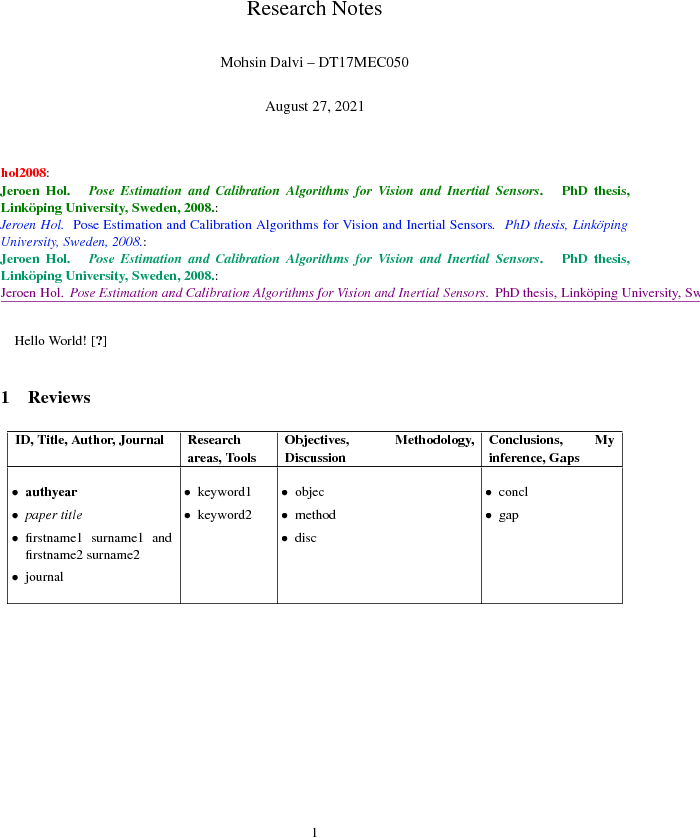
\includegraphics{image1}%
%
\hskip 10pt % insert a non-breaking space of specified width.
%
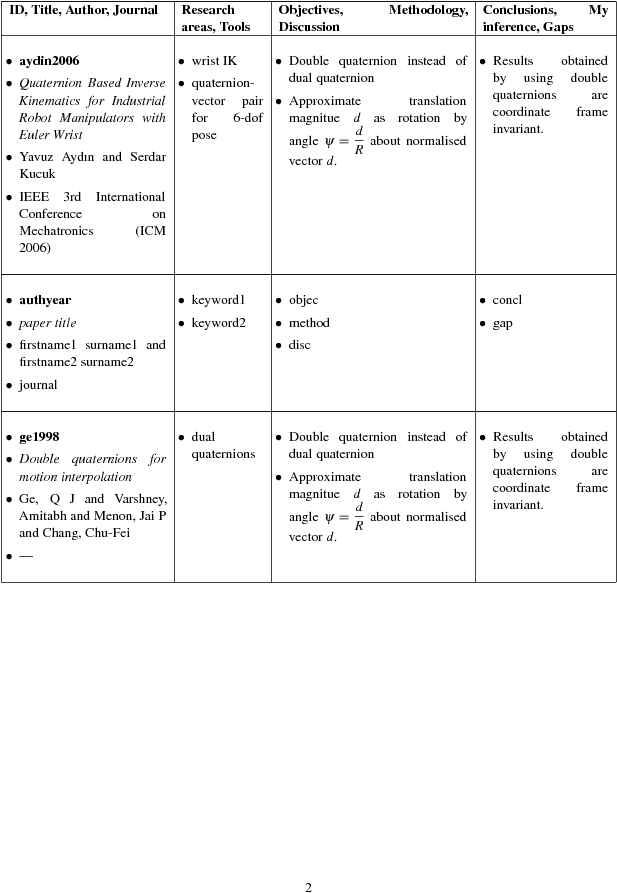
\includegraphics{image2}
\end{codeexample}
%
to place two graphics next to each other. This here is just the same (except
that our graphics occupy more code in the |.tex| file).

Note that there is also a comment sign after |\end{tikzpicture}|. This is not
just a best practice: it is necessary to suppress spurious spaces! In \TeX{},
every newline character is automatically converted to a white space (unless you
have an empty line, of course). In our case, we want no white spaces.

In our second picture, we see the effects of switch our math expression to
constant definitions as promised earlier. The interesting part starts with two
constants which are defined by means of two |\newcommand|s: we define |\MU| to
be 0 and |\SIGMA| to be |1e-3|. This is one way to define constants (note that
such a definition of constants should probably introduce round braces if
numbers are negative, i.e.\@ something like |\newcommand\negative{(-4)}|).


\subsection{Fixing the Vertical Alignment and Adjusting Tick Label Positions}
\label{sec:tut1:step4}

Note that even though our individual pictures look quite good, the combination
of both is not properly aligned. The experienced reader identifies the weak
point immediately: the bounding box of the two images differs, and they are
aligned at their baseline (which is the bottom edge of the picture). In
particular, the |xlabel=$x$| of the left picture and the automatically inserted
scaling label |\cdot 10^{-3}| of the right picture cause an unwanted vertical
shift. We want to fix that in the next step.

Besides the bad alignment, we find it a little bit misleading that the axis
descriptions of the second picture are between both pictures. We would like to
move them to the right.

Let us present the result first:
%
\begin{codeexample}[]
\begin{tikzpicture}[baseline]
    \begin{axis}[
        title=Inv. cum. normal,
        xlabel={$x$},
        ylabel={$y$},
        ymin=-3, ymax=3,
        minor y tick num=1,
    ]
        \addplot [blue] table {invcum.dat};
    \end{axis}
\end{tikzpicture}%
%
\hskip 10pt % insert a non-breaking space of specified width.
%
\begin{tikzpicture}[baseline]
    \begin{axis}[
        yticklabel pos=upper,
    ]
        % density of Normal distribution:
            \newcommand\MU{0}
            \newcommand\SIGMA{1e-3}
        \addplot [red,domain=-3*\SIGMA:3*\SIGMA,samples=201]
            {exp(-(x-\MU)^2 / 2 / \SIGMA^2) / (\SIGMA * sqrt(2*pi))};
    \end{axis}
\end{tikzpicture}
\end{codeexample}
%
This listing has a couple of modifications. The most important one is the we
added an option list to the |tikzpicture| environment: the |baseline| option.
This option shifts the picture up or down such that the canvas coordinate $y=0$
is aligned at the baseline of the surrounding text. In \PGFPlots{}, the $y=0$
line is the lower edge of the box. This simple feature allows both axes to be
aligned vertically: now, their boxes are aligned rather than the lower edges of
their bounding boxes. The option baseline needs to be provided to all pictures
for which this shifting should be done -- in our case, to all which are to be
placed in one row. Keep in mind that it is an option for |\begin{tikzpicture}|.

The second change is rather simple: we only added the option
|yticklabel pos=upper| to the second axis. This moves all tick labels to the
right, without changing anything else.

Note that there is much more to say about alignment and bounding box control.
After all, we did not really change the bounding box -- we simply moved the
pictures up or down. There is also the use case where we want horizontal
alignment: for example if the two pictures should be centered horizontally or
if they should be aligned with the left- and right end of the margins. The
associated keys |\begin{tikzpicture}[trim axis left, trim axis right]| and
|\centering| are beyond the scope of this tutorial, please refer to
Section~\ref{pgfplots:sec:align} for details.


\subsection{Satisfying Different Tastes}
\label{sec:tut1:step5}

We are now in a position where the figures as such are in a good shape.

However, an increase in knowledge will naturally lead to an increase in
questions. Some of these questions will be part of other how-to lectures. But
the most commonly asked questions are addressed here (feel free to email some
more if you believe that I should include another hotspot):
%
\begin{enumerate}
    \item How can I get rid of that $10^{-3}$ label?
    \item How can I modify the number printing?
    \item How can I have one single line per axis rather than a box?
\end{enumerate}

This here gives brief hints where to look in this reference manual for more
details. We modify the appearance of the second picture according to the
questions above:
%
\begin{codeexample}[]
\begin{tikzpicture}
\begin{axis}[
    axis lines=left,
    scaled ticks=false,
    xticklabel style={
        rotate=90,
        anchor=east,
        /pgf/number format/precision=3,
        /pgf/number format/fixed,
        /pgf/number format/fixed zerofill,
    },
]
    % density of Normal distribution:
        \newcommand\MU{0}
        \newcommand\SIGMA{1e-3}
  \addplot [red,domain=-3*\SIGMA:3*\SIGMA,samples=201]
        {exp(-(x-\MU)^2 / 2 / \SIGMA^2)
            / (\SIGMA * sqrt(2*pi))};
\end{axis}
\end{tikzpicture}
\end{codeexample}

The appearance of the axes as such can be controlled by means of the
|axis lines| key. It accepts the values |left, right, box, center, none| (and
also |top, bottom, middle| which are aliases). The |xticklabel style| key
modifies a predefined style (note the use of indentation here!). A style is a
collection of keys which are applied in a specific context. Styles are very
useful and are widely used by \PGFPlots{}. In our case, we adjust a couple of
options like rotation, alignment (the |anchor| option), and number printing
options. The precise details of these individual options is beyond the scope of
this tutorial. The keys actually belong to \Tikz{} -- and the \Tikz{} manual is
the reference for these keys (although \PGFPlots{} also covers most of the
topics). The complete set of number printing options is available in both the
\Tikz{} manual~\cite{tikz} and the manual for \PGFPlotstable{} which is shipped
with \PGFPlots{}. A brief extract can be found in
Section~\ref{sec:number:printing}.


\subsection{Finishing Touches: Automatic Generation of Individual Pdf Graphics}
\label{sec:tut1:step6}

As last step in this lecture, I would like to talk about one technical topic.
Typically, a \TeX{} document starts quite simple: a little bit of text, perhaps
one or two pictures. But they tend to grow. And eventually, you will encounter
one of the weak points of \PGFPlots{}: the graphics are involved and \TeX{}
consumes a lot of time to generate them. Especially if it keeps regenerating
them even though they did not change at all. The fact that we need to rerun the
pdflatex processor all the time makes things worse.

Fortunately, there are solutions. A simple solution is: why can't we write each
individual graphics into a separate |.pdf| file and use |\includegraphics| to
include it!? The answer is: yes, we can. And it is surprisingly simple to do
so.

In order to convert every |tikzpicture| environment automatically to an
external graphics \emph{without} changing any line of code in the \TeX{} file,
we can simply write the following two lines into the document's preamble:
%
\begin{codeexample}[code only]
\usepgfplotslibrary{external}
\tikzexternalize

...
\begin{document}
...
\end{document}
\end{codeexample}
%
But now, we \emph{have to provide a command line switch to pdflatex}:
%
\begin{codeexample}[code only]
pdflatex -shell-escape myfile.tex
\end{codeexample}

This works out of the box with |pdflatex|. If you use |latex/dvips|,
|lualatex|, |dvipdfm| or any other \TeX{} derivatives, you need to modify the
option |\tikzexternalize[system call=...]| (which is, unfortunately,
system-dependent, especially for the postscript variants).

It might be too much to discuss how to define individual file names or how to
modify the file name generation strategy. There is also the
|\tikzexternalize[mode=list and make]| feature which generates a GNU Make file
to allow |\label/\ref| to things inside of the external graphics and which
supports the generation of all images in parallel (if you have a multi-core
PC).

Details of the |external| library can be found in
Section~\ref{sec:pgfplots:export} (but only a brief survey) and, in all depth,
in the \Tikz{} reference manual~\cite{tikz}.


\subsection{Summary}

We learned how to create a standard axis, and how to assign basic axis
descriptions. We also saw how to plot functions from a data table (in our case
a tab-separated file, but other delimiters as in CSV files are also supported)
and from math expressions. We saw that \PGFPlots{} does a reasonable good job
at creating a fully-featured axis automatically (like scaling the units
properly, choosing tick positions and labels). We also learned how to improve
vertical alignment and how to customize the appearance of an axis.

Next steps might be how to draw multiple plots into the same axis, how to
employ scatter plots of \PGFPlots{}, how to generate logarithmic axes, or how
to draw functions of two variables. Some of these aspects will be part of
further how-to lectures.


\section{Solving a Real Use Case: Scientific Data Analysis}

In this section, we assume that you did some scientific experiment. The
scientific experiment yielded three input data tables: one table for each
involved parameter $d=2$, $d=3$, $d=4$. The data tables contain ``degrees of
freedom'' and some accuracy measurement ``|l2_err|''. In addition, they might
contain some meta-data (in our case a column ``level''). For example, the data
table for $d=2$ might be stored in |data_d2.dat| and may contain
%
\begin{codeexample}[code only]
dof        l2_err     level
5          8.312e-02  2
17         2.547e-02  3
49         7.407e-03  4
129        2.102e-03  5
321        5.874e-04  6
769        1.623e-04  7
1793       4.442e-05  8
4097       1.207e-05  9
9217       3.261e-06  10
\end{codeexample}
%
The other two tables are similar, we provide them here to simplify the
reproduction of the examples. The table for $d=3$ is stored in |data_d3.dat|,
it is
%
\begin{codeexample}[code only]
dof        l2_err     level
7          8.472e-02  2
31         3.044e-02  3
111        1.022e-02  4
351        3.303e-03  5
1023       1.039e-03  6
2815       3.196e-04  7
7423       9.658e-05  8
18943      2.873e-05  9
47103      8.437e-06  10
\end{codeexample}
%
Finally, the last table is |data_d4.dat|
%
\begin{codeexample}[code only]
dof        l2_err     level
9          7.881e-02  2
49         3.243e-02  3
209        1.232e-02  4
769        4.454e-03  5
2561       1.551e-03  6
7937       5.236e-04  7
23297      1.723e-04  8
65537      5.545e-05  9
178177     1.751e-05  10
\end{codeexample}

What we want is to produce three plots, each dof versus |l2_err|, in a loglog
plot. We expect that the result is a line in a log--log plot, and we are
interested in its slope $\log e(N) = -a \log(N)$ because that characterizes our
experiment.


\subsection{Getting the Data into \TeX{}}
\label{sec:tut2:step1}

Our first step is to get one of our data tables into \PGFPlots{}. In addition,
we want axis descriptions for the $x$- and $y$-axes and a title on top of the
plot.

Our first version looks like
%
\begin{codeexample}[]
%\documentclass{article}
%\usepackage{pgfplots}
%\pgfplotsset{compat=1.5}

%\begin{document}

\begin{tikzpicture}
\begin{loglogaxis}[
    title=Convergence Plot,
    xlabel={Degrees of freedom},
    ylabel={$L_2$ Error},
]
    \addplot table {data_d2.dat};
\end{loglogaxis}
\end{tikzpicture}

%\end{document}
\end{codeexample}

Our example is similar to that of the lecture in Section~\ref{sec:tut1:step1}
in that it defines some basic axis descriptions by means of |title|, |xlabel|,
and |ylabel| and provides data using |\addplot table|. The only difference is
that we used |\begin{loglogaxis}| instead of |\begin{axis}| in order to
configure logarithmic scales on both axes. Note furthermore that we omitted any
options after |\addplot|. As explained in Section~\ref{sec:tut1:step1}, this
tells \PGFPlots{} to consult its |cycle list| to determine a suitable option
list.


\subsection{Adding the Remaining Data Files of Our Example.}
\label{sec:tut2:step2}

\PGFPlots{} accepts more than one |\addplot ... ;| command -- so we can just
add our remaining data files:
%
\begin{codeexample}[]
\begin{tikzpicture}
\begin{loglogaxis}[
    title=Convergence Plot,
    xlabel={Degrees of freedom},
    ylabel={$L_2$ Error},
]
    \addplot table {data_d2.dat};
    \addplot table {data_d3.dat};
    \addplot table {data_d4.dat};
\end{loglogaxis}
\end{tikzpicture}
\end{codeexample}

You might wonder how \PGFPlots{} chose the different line styles. And you might
wonder how to modify them. Well, if you simply write |\addplot| without options
in square brackets, \PGFPlots{} will automatically choose styles for that
specific plot. Here ``automatically'' means that it will consult its current
|cycle list|: a list of predefined styles such that every |\addplot| statement
receives one of these styles. This list is customizable to a high degree.

Instead of the |cycle list|, you can easily provide style options manually. If
you write

|\addplot[|\meta{options}|] ...|,

\PGFPlots{} will only use \meta{options} and will ignore its |cycle list|. If
you write a plus sign before the square brackets as in

|\addplot+[|\meta{options}|] ...|,

\PGFPlots{} will append \meta{options} to the automatically assigned cycle
list.


\subsection{Add a Legend and a Grid}
\label{sec:tut2:step3}

A legend is a text label explaining what the plots are. A legend can be
provided for one or more |\addplot| statements using the |legend entries| key:
%
\begin{codeexample}[]
\begin{tikzpicture}
\begin{loglogaxis}[
    title=Convergence Plot,
    xlabel={Degrees of freedom},
    ylabel={$L_2$ Error},
    grid=major,
    legend entries={$d=2$,$d=3$,$d=4$},
]
    \addplot table {data_d2.dat};
    \addplot table {data_d3.dat};
    \addplot table {data_d4.dat};
\end{loglogaxis}
\end{tikzpicture}
\end{codeexample}
%
Here, we assigned a comma-separated list of text labels, one for each of our
|\addplot| instructions. Note the use of math mode in the text labels. Note
that if any of your labels contains a comma, you have to surround the entry by
curly braces. For example, we could have used
|legend entries={{$d=2$},{$d=3$},{$d=4$}}| -- \PGFPlots{} uses these braces to
delimit arguments and strips them afterwards (this holds for any option, by the
way).

Our example also contains grid lines for which we used the |grid=major| key. It
activates major grid lines in all axes.

You might wonder how the text labels map to |\addplot| instructions. Well, they
are mapped by index. The first label is assigned to the first plot, the second
label to the second plot and so on. You can exclude plots from this counting if
you add the |forget plot| option to the plot (using |\addplot+[forget plot]|,
for example). Such plots are excluded from both cycle lists and legends.


\subsection{Add a Selected Fit-line}
\label{sec:tut2:step4}

Occasionally, one needs to compute linear regression lines through input
samples. Let us assume that we want to compute a fit line for the data in our
fourth data table (|data_d4.dat|). However, we assume that the interesting part
of the plot happens if the number of degrees of freedom reaches some asymptotic
limit (i.e.\@ is very large). Consequently, we want to assign a high
uncertainty to the first points when computing the fit line.

\PGFPlots{} offers to combine table input and mathematical expressions (note
that you can also type pure mathematic expressions, although this is beyond the
scope of this example). In our case, we employ this feature to create a
completely new column -- the linear regression line:

\begin{codeexample}[]
%\usepackage{pgfplotstable}
%...
\begin{tikzpicture}
\begin{loglogaxis}[
    title=Convergence Plot,
    xlabel={Degrees of freedom},
    ylabel={$L_2$ Error},
    grid=major,
    legend entries={$d=2$,$d=3$,$d=4$},
]
    \addplot table {data_d2.dat};
    \addplot table {data_d3.dat};
    \addplot table {data_d4.dat};
    \addplot table [
      x=dof,
      y={create col/linear regression={y=l2_err,
       variance list={1000,800,600,500,400,200,100}}}]
        {data_d4.dat};
\end{loglogaxis}
\end{tikzpicture}
\end{codeexample}

Note that we added a further package: |pgfplotstable|. It allows to postprocess
tables (among other things. It also has a powerful table typesetting toolbox
which rounds and formats numbers based on your input CSV file).

Here, we added a fourth plot to our axis. The first plot is also an
|\addplot table| statement as before -- and we see that it loads the data file
|data_d4.dat| just like the plot before. However, it has special keys which
control the coordinate input: |x=dof| means to load x coordinates from the
column named ``dof''. This is essentially the same as in all of our other plots
(because the ``dof'' column is the first column). It also uses
|y={create col/...}|. This lengthy statement defines a completely new column.
The |create col/linear regression| prefix is a key which can be used whenever
new table columns can be generated. As soon as the table is queried for the
first time, the statement is evaluated and then used for all subsequent rows.
The argument list for |create col/linear regression| contains the column name
for the function values |y=l2_err| which are to be used for the regression line
(the x arguments are deduced from |x=dof| as you guessed correctly). The
|variance list| option is optional. We use it to assign variances
(uncertainties) to the first input points. More precisely: the first
encountered data point receives a variance of 1000, the second 800, the third
600, and so on. The number of variances does not need to match up with the
number of points; \PGFPlots{} simply matches them with the first encountered
coordinates.

Note that since our |legend entries| key contains only three values, the
regression line has no legend entry. We could easily add one, if we wanted. We
can also use |\addplot+[forget plot] table[...]| to explicitly suppress the
generation of a legend as mentioned above.

Whenever \PGFPlots{} encounters mathematical expressions, it uses its built-in
floating point unit. Consequently, it has a very high data range -- and a
reasonable precision as well.


\subsection{Add an Annotation using \Tikz{}: a Slope Triangle}
\label{sec:tut2:step5}

Often, data requires interpretation -- and you may want to highlight particular
items in your plots. This ``highlight particular items'' requires to draw into
an axis, and it requires a high degree of flexibility. Users of \Tikz{} would
say that \Tikz{} is a natural choice -- and it is.

In our use case, we are interested in slopes. We may want to compare slopes of
different experiments. And we may want to show selected absolute values of
slopes.

Here, we use \Tikz{} to add custom annotations into a \PGFPlots{} axis. We
choose a particular type of a custom annotation: we want to mark two points on
a line plot. One way to do so would be to determine the exact coordinates and
to place a graphical element at this coordinate (which is possible using
|\draw ... (1e4,1e-5) ... ;|). Another (probably simpler) way is to use the
|pos| feature to identify a position ``25\% after the line started''.

Based on the result of Section~\ref{sec:tut2:step4}, we find
%
\begin{codeexample}[]
%\usepackage{pgfplotstable}
%...
\begin{tikzpicture}
\begin{loglogaxis}[
    title=Convergence Plot,
    xlabel={Degrees of freedom},
    ylabel={$L_2$ Error},
    grid=major,
    legend entries={$d=2$,$d=3$,$d=4$},
]
    \addplot table {data_d2.dat};
    \addplot table {data_d3.dat};
    \addplot table {data_d4.dat};
    \addplot table [
      x=dof,
      y={create col/linear regression={y=l2_err,
       variance list={1000,800,600,500,400,200,100}}}]
        {data_d4.dat}
            % save two points on the regression line
            % for drawing the slope triangle
            coordinate [pos=0.25] (A)
            coordinate [pos=0.4]  (B)
   ;
    % save the slope parameter:
    \xdef\slope{\pgfplotstableregressiona}

    % draw the opposite and adjacent sides
    % of the triangle
    \draw (A) -| (B)
         node [pos=0.75,anchor=west]
         {\pgfmathprintnumber{\slope}};
\end{loglogaxis}
\end{tikzpicture}
\end{codeexample}

The example is already quite involved since we added complexity in every step.
Before we dive into the details, let us take a look at a simpler example:
%
\begin{codeexample}[]
\begin{tikzpicture}
\begin{loglogaxis}
    \addplot table {data_d2.dat}
       coordinate [pos=0.25] (A)
       coordinate [pos=0.4]  (B)
    ;

    \draw [-stealth] (A) -| (B);

    \node [pin=0:Special.] at (769,1.623e-04) {};
\end{loglogaxis}
\end{tikzpicture}
\end{codeexample}
%
Here, we see two annotation concepts offered by \PGFPlots{}: the first is to
insert drawing commands right after an |\addplot| command (but before the
closing semicolon). The second is to add standard \Tikz{} commands, but use
designated \PGFPlots{} coordinates. Both are \Tikz{} concepts. The first is
what we want here: we want to identify two coordinates which are ``somewhere''
on the line. In our case, we define two named coordinates: coordinate $A$ at
25\% of the line and coordinate $B$ at 40\% of the line. Then, we use
\verb#\draw (A) -| (B)# to draw a triangle between these two points. The second
is only useful if we know some absolute coordinates in advance.

Coming back to our initial approach with the regression line, we see that it
uses the first concept: it introduces named coordinates after |\addplot|, but
before the closing semicolon. The statement |\xdef\slope| introduces a new
macro. It contains the (expanded due to the ``eXpanded DEFinition'') value of
|\pgfplotstableregressiona| which is the slope of the regression line. In
addition to the slope triangle, we also add a node in which we typeset that
value using |\pgfmathprintnumber|.

Note that the example above is actual a ``happy case'': it can happen easily
that labels which are added inside of the axis environment are clipped away:
%
\begin{codeexample}[]
\begin{tikzpicture}
\begin{loglogaxis}[
    tiny,
]
    \addplot table {data_d2.dat}
        node [pos=1,pin=0:Special.] {}
    ;
\end{loglogaxis}
\end{tikzpicture}
\end{codeexample}
%
The example above combines the |pos| label placement with the node's label.
Note that the small style |tiny| installs a \PGFPlots{} preset which is better
suited for very small plots -- it is one of the many supported scaling
parameters. The problem here is apparent: the text of our extra node is clipped
away. Depending on your data, you have a couple of solutions here:
%
\begin{itemize}
    \item use |clip=false| to disable clipping of plot paths at all,
    \item use |clip mode=individual| to enable clipping only for plot paths,
    \item draw the node outside of the axis environment but inside of the
        picture environment.
\end{itemize}
%
The first attempt works quite well for most figures:
%
\begin{codeexample}[]
\begin{tikzpicture}
\begin{loglogaxis}[
    tiny,
    clip=false,
]
    \addplot table {data_d2.dat}
        node [pos=1,pin=0:Special.] {}
    ;
\end{loglogaxis}
\end{tikzpicture}
\end{codeexample}
%
Note that this approach in which the nodes are placed before the closing
semicolon implies that nodes inherit the axis line style and color.


\subsection{Summary}

We learned how to define a (logarithmic) axis, and how to assign basic axis
descriptions. We also saw once more how to use one or more |\addplot table|
commands to load table data into \PGFPlots{}. We took a brief look into
regression and \Tikz{} drawing annotations.

We also encountered the |tiny| style which is one of the ways to customize the
size of an axis. Others are |width|, |height|, the other predefined size styles
like |normalsize|, |small|, or |footnotesize|, and the two different scaling
modes |/pgfplots/scale| and |/tikz/scale| (the first scales only the axis, the
second also the labels).

Next steps might be how to visualize functions using line plots, how to align
adjacent graphics properly (even if the axis descriptions vary), how to employ
scatter plots of \PGFPlots{}, or how to draw functions of two variables.

%The steps are explained in all detail in the reference
%Chapter~\ref{cha:pgfplots:reference}.


\section{Use Cases involving Scatter Plots}

Assuming that we are more or less familiar with the basics of the preceding
tutorials, we would like to draw a scatter plot. A scatter plot is one in which
markers indicate the important information.

There are many different kinds of scatter plots and this section covers a
couple of them.

\subsection{Scatter Plot Use Case A}
\label{sec:tut3:usecaseA}

In this subsection, we address the following scatter plot use case: assume that
we are given a couple of special $(x,y)$ coordinates along with color data at
every vertex. We would like to draw markers at the positions and choose
individual colors depending on the color data.


\subsubsection{Importing the Data File}

We assume that our input data is given as a table containing much more columns
than we need. The first couple of rows are as follows:

    \lstinputlisting[
        columns=fixed,
        breaklines=false,
        tabsize=15,
        lastline=8,
            ]{plotdata/concat_VV_together_grid.dat}

What we need is the first and second column to get the $x$- and $y$-coordinate
values, respectively, and the third column |f(x)| to choose color values. The
color values are very small and have a high range: there are values of order
$10^{-6}$ and there are values of order $1$. Such ranges are best shown on a
logarithmic scale, which is why we will resort to some logarithmic scale on the
absolute values of this column. Thus, a requirement will be to accept a math
expression (involving logs) on the color data column.

Note that the data file (and all others referenced in this manual) are shipped
with \PGFPlots{}; you can find them in the subfolder
\texttt{doc/latex/pgfplots/plotdata}.

We learned already how to read table data from a file, so our first step is
relatively straightforward.

\begin{codeexample}[]
\begin{tikzpicture}
\begin{axis}
    \addplot+ [only marks] table
        {concat_VV_together_grid.dat};
\end{axis}
\end{tikzpicture}
\end{codeexample}

Here, the only non-trivial variation is the option |only marks| which is given
after the plus sign. Keep in mind that |\addplot+[|\meta{options}|]| means that
\PGFPlots{} shall combine the set of options of its |cycle list| with
\meta{options}. In our case, |only marks| does what it says. The |only marks|
plot handler is the most simple scatter plot: it uses the same color for every
marker.

Note that |\addplot table| takes the first column as |x| and the second as |y|
(which matches our input file perfectly).


\subsubsection{Fine Tuning}

We agree that our initial import has unsuitable displayed limits: there is too
much white space around the interesting plot area. In addition, the markers
overlap because they are too large. We can modify the appearance as follows:

\begin{codeexample}[]
\begin{tikzpicture}
\begin{axis}[
    enlargelimits=false,
]
    \addplot+ [only marks,mark size=0.6pt]
        table {concat_VV_together_grid.dat};
\end{axis}
\end{tikzpicture}
\end{codeexample}

As before, we assume that we add more options after |\begin{axis}|.
Consequently, we introduced suitable indentation and a trailing comma after the
option. Note that |enlargelimits| is typically active; it means that
\PGFPlots{} increases the displayed range by $10\%$ by default. Deactivating it
produces tight limits according to the input data.

Our second option is |mark size| -- using an absolute size (about the radius or
half size of the marker).


\subsubsection{Color Coding According To Input Data}

We are quite close to our goal, except for the colors. As discussed, our input
file contains three columns and the third one should be used to provide color
information. In our case, the data file has a column named |f(x)|.
%
\begin{codeexample}[]
\begin{tikzpicture}
    \begin{axis}[
        enlargelimits=false,
        colorbar,
    ]
        \addplot+ [
            only marks,
            scatter,
            point meta={
                ln(1e-6+abs(\thisrow{f(x)}))/ln(10)
            },
            mark size=0.6pt,
        ] table {concat_VV_together_grid.dat};
    \end{axis}
\end{tikzpicture}
\end{codeexample}
%
We added a couple of options to our example: the options |scatter|, and
|point meta|, |colorbar|. The option |scatter| has a slightly misleading name as
we already had a scatter plot before we added that option. It activates scatter
plots with individual appearance: without further options, it chooses
individual colors for every marker. The ``individual colors'' are based on
something which is called ``|point meta|'' in \PGFPlots{}. The |point meta| is
typically a scalar value for every input coordinate. In the default
configuration, it is interpreted as ``color data'' for the coordinate in
question. This also explains the other option: |point meta=...| tells
\PGFPlots{} which values are to be used to determine colors. Note that the
default value of |point meta| is to use the $y$~coordinate. In our case, we
have a complicated math expression which is related to our input file: it
contains small quantities in column |f(x)| which are based shown on a
logarithmic scale as their differ over a huge range. Since a logarithm must not
have a non-positive argument, we have $10^{-6} + \text{abs}(\dotsb)$ as
expression which ensures that the argument is never smaller than |10^{-6}| and
that is is positive. The divider |/ln(10)| means that we have logarithms
base~$10$. But the key point of the whole complicated expression can be
summarized as follows:
%
\begin{enumerate}
    \item We can use |\thisrow|\marg{column name} to refer to table columns.
        Here, ``this row'' means to evaluate the table for the ``data point
        which is being read from the current row''.
    \item We can combine |\thisrow| with any complicated math expression.
\end{enumerate}
%
The third new option |colorbar| activates the color bar on the right hand side
(as you guessed correctly). We see that the smallest value is $-6$ which
corresponds to our value |1e-6| in the math expression.

You might wonder how a scalar value (the number stored in the |f(x)| column)
results in a color. \PGFPlots{} computes the minimum and maximum value of all
such numbers. Then, it maps every number into a |colormap|. A |colormap|
defines a couple of colors and interpolates linearly between such colors. That
means that the smallest value of |point meta| is mapped to the first color in a
|colormap| whereas the largest value of |point meta| is mapped to the last
color in the |colormap|. All others are mapped to something in-between.

More information about |colormap| and |point meta| can be found in
Section~\ref{sec:colormap:input:format} and in
Section~\ref{pgfplots:point:meta}.


\subsection{Scatter Plot Use Case B}

As already mentioned, there are various use cases for scatter plots. The
default configuration of the |scatter| key is to read numeric values of
|point meta| and choose colors by mapping that value into the current |colormap|.

A different application would be to expect symbolic input (some string) and
choose different markers depending on that input symbol.

Suppose that you are given a sequence of input coordinates of the form $(x,y)$
\meta{class label} and that you want to choose marker options depending on the
\meta{class label}. A \PGFPlots{} solution could be
%
\begin{codeexample}[]
\begin{tikzpicture}
\begin{axis}
    \addplot [
        scatter,
        only marks,
        point meta=explicit symbolic,
        scatter/classes={
            a={mark=square*,blue},
            b={mark=triangle*,red},
            c={mark=o,draw=black}% <-- don't add comma
        },
    ] table [meta=label] {
        x      y        label
        0.1    0.15     a
        0.45   0.27     c
        0.02   0.17     a
        0.06   0.1      a
        0.9    0.5      b
        0.5    0.3      c
        0.85   0.52     b
        0.12   0.05     a
        0.73   0.45     b
        0.53   0.25     c
        0.76   0.5      b
        0.55   0.32     c
    };
\end{axis}
\end{tikzpicture}
\end{codeexample}
%
As in our previous use case in Section~\ref{sec:tut3:usecaseA}, we have the
options |scatter|, |only marks|, and a configuration how to retrieve the
|point meta| values by means of the |meta| key. One new key is
|point meta=explicit symbolic|: it tells \PGFPlots{} that any encountered values
of |point meta| are to be interpreted as string symbols. Furthermore, it tells
\PGFPlots{} that the every input coordinate comes with an explicit value (as
opposed to a common math expression, for example). The other different option
is |scatter/classes|. As you guessed from the listing, it is a map from string
symbol to marker option list. This allows to address such use cases in a simple
way.

This example has actually been replicated from the reference manual section for
|scatter/classes|.


\subsection{Scatter Plot Use Case C}

Finally, this tutorial sketches a further use case for scatter plots: given a
sequence of coordinates $(x,y)$ with individual string labels, we want to draw
the string label at the designated positions.

This can be implemented by means of the |nodes near coords| feature of
\PGFPlots{}, which is actually based on |scatter|:
%
\begin{codeexample}[]
\begin{tikzpicture}
\begin{axis}[
    enlargelimits=0.2,
]
    \addplot+ [nodes near coords,only marks,
       point meta=explicit symbolic]
    table [meta=label] {
        x    y   label
        0.5  0.2 1
        0.2  0.1 t2
        0.7  0.6 3
        0.35 0.4 Y4
        0.65 0.1 5
    };
\end{axis}
\end{tikzpicture}
\end{codeexample}
%
In this case, we have |point meta=explicit symbolic| in order to express the
fact that our labels are of textual form (see the reference manual section for
|nodes near coords| for applications of \emph{numeric} labels). The remaining
stuff is done by the implementation of |nodes near coords|. Note that enlarged
the axis limits somewhat in order to include the text nodes in the visible
area.

There is much more to say about |scatter| plots, and about |nodes near coords|.
Please consider this subsection as a brief pointer to
Section~\ref{sec:pgfplots:scatter:2d} in the reference manual.


\subsection{Summary}

We learned how to generate scatter plots with single color using |only marks|,
scatter plots with individually colored markers using the |scatter| key,
scatter plots with specific marker styles depending on some class label using
|scatter/classes| and text nodes using |nodes near coords|.

Furthermore, we introduced the concept of ``|point meta| data'': once as
(scalar valued) color data, once as symbolic class label and once as text
label.

There is much more to say, especially about |point meta| which is introduced
and explained in all depth in Section~\ref{pgfplots:point:meta}.

There is also more to say about |scatter| plots, for example how to generate
scatter plots with individually sized markers and/or colors (by relying on
|\pgfplotspointmetatransformed|, see the reference manual section for
|visualization depends on|). In addition, |scatter| plots can be customized to
a high degree which is explained in Section~\ref{sec:pgfplots:scatter:2d}.


\section{Solving a Real Use Case: Functions of Two Variables}

In this tutorial, we assume that we have two functions for which we seek a
plot: the first is a sampled function given by a huge data file and the second
is the math expression $g(x,y)=\exp(-x^2-y^2)\cdot x$.

Our first function actually consists of two data files: the first file contains
some scattered data which resembles a discretization (``sampling'') of a
function and the second file contains data for the function as such, sampled on
a lattice. Our requirement here is two draw \emph{two} graphs into the same
axis: one in which the function is plotted as a smooth, colored surface and one
in which the scattered data file should be on top of the surface because it
provides more detail how the function was represented in the computer.

The second function which is given as math expression should be visualized
using a contour plot. A contour plot expects some fixed values $g_1, \dotsc,
g_k$ as input (the contour values) and plots one curve for each $g_j = g(x,y)$
(i.e.\@ if you go hiking without ever changing the height of your path).


\subsection{Surface Plot from Data File}

Our first step is to load the data file and to plot a surface.

Clearly, functions of two variables require a more sophisticated input format:
they are typically sampled on a unified grid with $n \times m$ points, i.e.\@
$n$~points for $x$ and $m$~points for $y$, resulting in a total of matrix with
$n\cdot m$ values $f_{ij} = f(x_i,y_i)$. How can we read matrix data? And what
if you have more than just the $z$ value? A standard way is to write the matrix
to a table, either in line by line ordering or in column by column ordering
(both are common).

Here, we assume that our function values are written to a table in which the
$y$ values vary from line to line. Here is an extract of the data file (which
is too large to list it here):

    \lstinputlisting[
        columns=fixed,
        breaklines=false,
        firstline=1,
        tabsize=15,
        lastline=6,
    ]{plotdata/concat_VV_together.dat}%
        \vskip-0.9\baselineskip
            $\vdots$
        \vskip-0.4\baselineskip
    \lstinputlisting[
        columns=fixed,
        breaklines=false,
        firstline=34,
        tabsize=15,
        lastline=43,
    ]{plotdata/concat_VV_together.dat}%
        \vskip-0.9\baselineskip
            $\vdots$

Note that the data file (and all others referenced in this manual) are shipped
with \PGFPlots{}; you can find them in the subfolder
\texttt{doc/latex/pgfplots/plotdata}.

The input file contains $x_0$, $x_1$, and $f(x_0,x_1)$ in columns named |x_0|,
|x_1|, and |f(x)|, respectively. In addition, it contains some meta data which
is irrelevant for us here.

Note that our input file contains \emph{empty lines} whenever |x_0| changes.
This is a common data format which simplifies the detection of ``scanline
length''. A scanline is one line in the input matrix, for example the line
consisting of all points with $x_0 = 0$. With such scanlines, \PGFPlots{} can
automatically deduce the size of the input matrix.

In order to plot the file as a surface, we proceed as in the previous example
by using |\addplot table|. However, we have to use |\addplot3| to indicate that
a three-dimensional result is expected: \pgfplotsexpensiveexample
%
\begin{codeexample}[]
\begin{tikzpicture}
\begin{axis}
    \addplot3 [
        surf,
        mesh/ordering=y varies,
    ] table {concat_VV_together.dat};
\end{axis}
\end{tikzpicture}
\end{codeexample}
%
The example looks familiar compared to our results of the preceding tutorials:
a |tikzpicture| environment containing an |axis| environment and the mentioned
|\addplot3| command. The option list contains |surf|, which tells \PGFPlots{}
how to visualize the input data. The key |mesh/ordering=y varies| tells
\PGFPlots{} how to decode the input matrix. This is important; otherwise
\PGFPlots{} would have chosen |x varies| which does not match our file.

Note that we there is no need to configure either |mesh/rows=|\meta{N} or
|mesh/cols=|\meta{N} here because these parameters are automatically deduced
from the scan line lengths marked by empty lines in our input file.

Since our |\addplot3 table| statement does not contain any hints which columns
should be plotted, \PGFPlots{} simply plots the first three columns against
each other.

The colors of a |surf| plot are chosen from the function values (unless you
configure some other value for |point meta|; this is similar to the scatter
plot example). In case of a function of two variables, the function value is
the third column.


\subsection{Fine-Tuning}

In order to stress how colors are to be mapped to values, we add a color bar to
our example from the previous subsection. In addition, we rotate the view a
little bit and add axis labels. Furthermore, we would like to have a smooth
color mapping.

We end up at
%
\pgfplotsexpensiveexample
\begin{codeexample}[]
\begin{tikzpicture}
\begin{axis}[
    view/h=40,
    colorbar horizontal,
    xlabel=$x$, ylabel=$y$,
]
    \addplot3 [
        surf,
        mesh/ordering=y varies,
        shader=interp,
    ] table {concat_VV_together.dat};
\end{axis}
\end{tikzpicture}
\end{codeexample}
%
Here, |view/h| rotates the ``horizontal'' parts of the view (only). It chooses
a new view angle for the orthographic projection. As you guessed, there is also
a |view/v| key and a |view=|\marg{h}\marg{v} variant.

The key |colorbar horizontal| is a style which activates a |colorbar| and
configures it to be displayed horizontally. The labels are placed using
|xlabel| and |ylabel| as we saw it before for visualizations of one-dimensional
functions. A colorbar uses the current |colormap| and adds axis descriptions to
show how values are mapped to colors.

 The |shader=interp| key activates a smooth color interpolation.


\subsection{Adding Scattered Data on Top of the Surface}

As motivated earlier, we have a second data set, one which characterizes how
the function has been represented in some computer simulation. We would like to
add the second data set as scatter plot on top of the function.

The data set as such is the very same as the one used in
Section~\ref{sec:tut3:usecaseA}, so we do not need to list it here again.
However, we have to include the two-dimensional scatter data into the
three-dimensional axis in a suitable way. We chose to place it on a fixed $z$
value as follows:
%
\pgfplotsexpensiveexample
\begin{codeexample}[]
\begin{tikzpicture}
\begin{axis}[
    view/h=40,
    colorbar horizontal,
    xlabel=$x$, ylabel=$y$,
]
    \addplot3 [surf,mesh/ordering=y varies,
        shader=interp
    ] table {concat_VV_together.dat};

    \addplot3 [blue,mark=*,
        mark options={fill=blue!80!black},
        only marks,mark size=0.6pt,
    ] table [z expr=1.2]{concat_VV_together_grid.dat};
\end{axis}
\end{tikzpicture}
\end{codeexample}
%
Now, we have two |\addplot3 table| statements in the same axis. None of them
uses the |cycle list| as we used explicit option lists. The first is our
surface plot. Note that it is plotted before the scatter plot: \PGFPlots{}
cannot handle depth information between adjacent |\addplot| statements. It
does, however, handle |z buffer| information for data of a single |\addplot|
statement. The second plot is our scatter plot: we recognize |only marks| and
|mark size| from Section~\ref{sec:tut3:usecaseA}. In addition, we configured
some color and marker options.

An important aspect is |\addplot3 table[z expr=1.2]| -- it tells \PGFPlots{}
how to choose $z$ values for the input file (otherwise, \PGFPlots{} would have
used the third column of that file). This is a convenient way to insert
two-dimensional data into a three-dimensional axis, provided you have
\emph{table} data. There is also a different way which works for both tables
and math expressions (or other input types). This different way is to install a
|z filter|, but that is beyond the scope of this tutorial for now.


\subsection{Computing a Contour Plot of a Math Expression}

This section addresses the second part of our use case example: a function of
two variables given by a math expression.

Our function of interest is $x \exp(-x^2-y^2)$. We start as in our tutorial for
one-dimensional functions given by a math expression (compare
Section~\ref{sec:tut1:step3}): by using an |\addplot| statement which is
followed by a math expression in curly braces. However, we rely on |\addplot3|
as in the preceding section:

\pgfplotsexpensiveexample
\begin{codeexample}[]
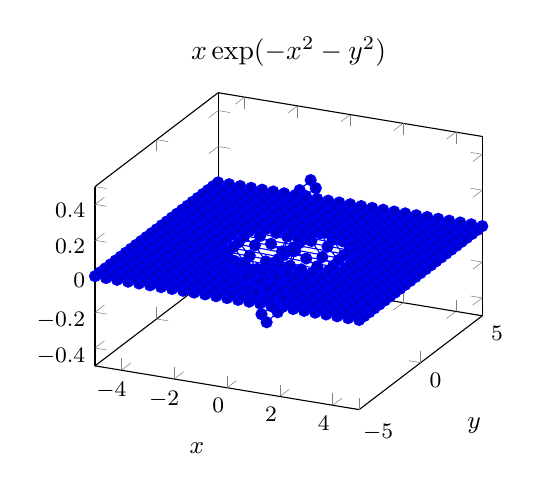
\begin{tikzpicture}
\begin{axis}[
    title={$x \exp(-x^2-y^2)$},
    xlabel=$x$, ylabel=$y$,
    small,
]
    \addplot3 {exp(-x^2-y^2)*x};
\end{axis}
\end{tikzpicture}
\end{codeexample}
%
Our example contains a basic axis environment with |title|, |xlabel|, |ylabel|
and the |small| key which are already known from the preceding tutorials. The
|\addplot3| has no options and is immediately followed by the math expression.
The absence of options tells \PGFPlots{} to rely on its |cycle list|. This, in
turn configures |mark=*| with |blue| color -- and a line plot. A line plot
combined with |\addplot3| is of limited use; it merely connects all incoming
points. Since points are sampled as a matrix (line by line). Our next step will
be to define a suitable plot handler.

Note, however, that our math expression depends on |x| and |y|. These two
variables are the sampling variables of \PGFPlots{} in its default configures:
both are sampled in the |domain| of interest using the correct number of
|samples|. The |\addplot3| statement takes care of computing $N\cdot M$ points
in the correct sequence where $N$ is the number of |samples| for $x$ and $M$ is
|samples y|, the number of samples used for $y$.

We can see that our sampling |domain| is too large. Switching to a smaller
|domain| focusses on the interesting parts of our function:

\pgfplotsexpensiveexample
\begin{codeexample}[]
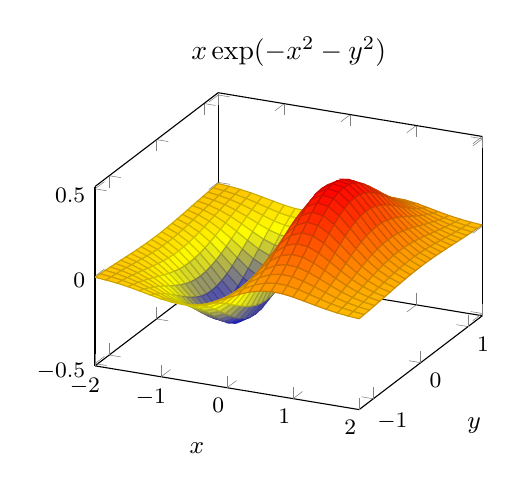
\begin{tikzpicture}
\begin{axis}[
    title={$x \exp(-x^2-y^2)$},
    xlabel=$x$, ylabel=$y$,
    small,
]
    \addplot3 [
        surf,
        domain=-2:2,
        domain y=-1.3:1.3,
    ] {exp(-x^2-y^2)*x};
\end{axis}
\end{tikzpicture}
\end{codeexample}
%
Here, we introduced an option list after |\addplot3|. Since we provided the
option list without the leading plus sign `|+|', \PGFPlots{} does not consider
its |cycle list| at all (and switches off |mark|s and the default color
settings). We added |domain| and |domain y| in order to restrict the sampling
domain in a suitable way. If we would have omitted |domain y|, the $y$ domain
would use the same value as the $x$ |domain|.

As you might have guessed, the |surf| key has the main use case of providing a
connection to the previous tutorial section: it is one of the natural
visualizations for functions of two variables. As in the preceding section, the
color has been deduced from the function value $z=f(x,y)$ (more precisely, by
relying on the default configuration |point meta=f(x)|).

The next step is to switch to contour plots by replacing `|surf|` by
`|contour lua|':

\pgfplotsexpensiveexample
\begin{codeexample}[]
\begin{tikzpicture}
\begin{axis}[
    title={$x \exp(-x^2-y^2)$},
    xlabel=$x$, ylabel=$y$,
    small,
]
    \addplot3 [
        contour lua,
        domain=-2:2,
        domain y=-1.3:1.3,
    ] {exp(-x^2-y^2)*x};
\end{axis}
\end{tikzpicture}
\end{codeexample}
%
Now, we have a contour plot -- although it is not quite what we had in mind.
First, there are so few contour lines that it is hard to see anything
(especially since the |line width| is too small). Furthermore, the |view|
direction is unfamiliar.

We add the |view| option with the argument for ``view from top'' and configure
the number of contour lines using the |contour/number| key and the |line width|
using the |thick| style:

\pgfplotsexpensiveexample
\begin{codeexample}[]
\begin{tikzpicture}
\begin{axis}[
    title={$x \exp(-x^2-y^2)$},
    enlarge x limits,
    view={0}{90},
    xlabel=$x$, ylabel=$y$,
    small,
	colorbar,
]
    \addplot3[
        domain=-2:2,
        domain y=-1.3:1.3,
        contour lua={number=14,labels=false},
        thick,
    ] {exp(-x^2-y^2)*x};
\end{axis}
\end{tikzpicture}
\end{codeexample}

This is what we wanted to achieve. Note that |contour lua| accepts options
which have the key prefix |contour/|. In this context, the prefix is optional.

Note that |contour lua| is different from almost all other plot handlers of
\PGFPlots{} with respect to one aspect: it requires you to invoke

|lualatex |\meta{texfilename}

\noindent instead of

|pdflatex |\meta{texfilename} .

\noindent 
The nonlinear algorithm to
compute contour lines is currently unavailable in plain \TeX{} which is stressed
by the name `|contour lua|'. 


If you cannot use |lualatex| for some reason, you can replace |contour lua| by |contour gnuplot|, provided that you have the external program |gnuplot| installed on your system (see the reference for |contour gnuplot| for more details).

\subsection{Summary}

We have sketched how to load a data table containing a sampled function of two
variables, and we learned how to visualize such data as |surf|ace plot. We
learned how to rotate the |view|, how to change the color |shader| of |surf|ace
plots, how to enabled |colorbar|s, and how to add |scatter| plots on top of
surface plots. Furthermore, we encountered the first contour plot as an example
for how to sample a function of two variables by means of built-in methods of
\PGFPlots{}.

It should be stressed that \PGFPlots{} needs no external tool to generate such
plots: every computer with a decent version of \PGFPlots{} can regenerate these plots.

There is more to say about three-dimensional axes, in particular regarding
|mesh/ordering|, parametric plots, perhaps line plots in three dimensions or
other plot types. Furthermore, there are some limitations regarding the
|z buffer|ing, i.e.\@ how \PGFPlots{} decides which parts of the figure are in
front of others. These items can be read in Section~\ref{sec:3d} and its
subsections.

You might also be interested in styles to change the appearance of a
three-dimensional axis, compare Section~\ref{sec:3d:axis:config}.

}%
